\documentclass{article}\usepackage[]{graphicx}\usepackage[]{xcolor}
% maxwidth is the original width if it is less than linewidth
% otherwise use linewidth (to make sure the graphics do not exceed the margin)
\makeatletter
\def\maxwidth{ %
  \ifdim\Gin@nat@width>\linewidth
    \linewidth
  \else
    \Gin@nat@width
  \fi
}
\makeatother

\definecolor{fgcolor}{rgb}{0.345, 0.345, 0.345}
\newcommand{\hlnum}[1]{\textcolor[rgb]{0.686,0.059,0.569}{#1}}%
\newcommand{\hlsng}[1]{\textcolor[rgb]{0.192,0.494,0.8}{#1}}%
\newcommand{\hlcom}[1]{\textcolor[rgb]{0.678,0.584,0.686}{\textit{#1}}}%
\newcommand{\hlopt}[1]{\textcolor[rgb]{0,0,0}{#1}}%
\newcommand{\hldef}[1]{\textcolor[rgb]{0.345,0.345,0.345}{#1}}%
\newcommand{\hlkwa}[1]{\textcolor[rgb]{0.161,0.373,0.58}{\textbf{#1}}}%
\newcommand{\hlkwb}[1]{\textcolor[rgb]{0.69,0.353,0.396}{#1}}%
\newcommand{\hlkwc}[1]{\textcolor[rgb]{0.333,0.667,0.333}{#1}}%
\newcommand{\hlkwd}[1]{\textcolor[rgb]{0.737,0.353,0.396}{\textbf{#1}}}%
\let\hlipl\hlkwb

\usepackage{framed}
\makeatletter
\newenvironment{kframe}{%
 \def\at@end@of@kframe{}%
 \ifinner\ifhmode%
  \def\at@end@of@kframe{\end{minipage}}%
  \begin{minipage}{\columnwidth}%
 \fi\fi%
 \def\FrameCommand##1{\hskip\@totalleftmargin \hskip-\fboxsep
 \colorbox{shadecolor}{##1}\hskip-\fboxsep
     % There is no \\@totalrightmargin, so:
     \hskip-\linewidth \hskip-\@totalleftmargin \hskip\columnwidth}%
 \MakeFramed {\advance\hsize-\width
   \@totalleftmargin\z@ \linewidth\hsize
   \@setminipage}}%
 {\par\unskip\endMakeFramed%
 \at@end@of@kframe}
\makeatother

\definecolor{shadecolor}{rgb}{.97, .97, .97}
\definecolor{messagecolor}{rgb}{0, 0, 0}
\definecolor{warningcolor}{rgb}{1, 0, 1}
\definecolor{errorcolor}{rgb}{1, 0, 0}
\newenvironment{knitrout}{}{} % an empty environment to be redefined in TeX

\usepackage{alltt}
\usepackage{amsmath} %This allows me to use the align functionality.
                     %If you find yourself trying to replicate
                     %something you found online, ensure you're
                     %loading the necessary packages!
\usepackage{amsfonts}%Math font
\usepackage{graphicx}%For including graphics
\usepackage{hyperref}%For Hyperlinks
\usepackage[shortlabels]{enumitem}% For enumerated lists with labels specified
                                  % We had to run tlmgr_install("enumitem") in R
\hypersetup{colorlinks = true,citecolor=black} %set citations to have black (not green) color
\usepackage{natbib}        %For the bibliography
\setlength{\bibsep}{0pt plus 0.3ex}
\bibliographystyle{apalike}%For the bibliography
\usepackage[margin=0.50in]{geometry}
\usepackage{float}
\usepackage{multicol}
%fix for figures
\usepackage{caption}
\newenvironment{Figure}
  {\par\medskip\noindent\minipage{\linewidth}}
  {\endminipage\par\medskip}
\IfFileExists{upquote.sty}{\usepackage{upquote}}{}
\begin{document}

\vspace{-1in}
\title{Lab 08 -- MATH 240 -- Computational Statistics}

\author{
  Brendan Mariano \\
  Colgate University  \\
  Mathematics  \\
  {\tt bmariano@colgate.edu}
}

\date{}

\maketitle

\begin{multicols}{2}
\begin{abstract}
This lab provides a template for understanding how a beta distribution works and for how we can find the optimal parameters to model a data set. We made conclusions about the beta distribution through analyzing it with various parameters and we fit it to data about death rates in 2022 using point estimators.

\end{abstract}

\noindent \textbf{Keywords:} beta distribution; density functions; samples; point estimation

\section{Introduction}
A beta distribution is a tool which can be used to model 


In this lab, we sought to determine whether the 
Provide an overarching summary of what you're talking about. In this section, you introduce the idea to the reader, and your goal is to pull them in. What's the mystery you aim to solve?

You want to provide enough background to understand the context of the work. Specifically, what is the question you are addressing? If it applies, describe what information currently exists about this problem, including citations, and explain how the question you're answering complements this work.

Provide a roadmap of the structure of the paper. 


\section{Density Functions and Parameters}
  A beta function is a distribution that is used to model set of data. Distribution's are useful because they allow us to model data to the best of our ability, which can allow us to make conclusions. The beta distribution specifically can take several different shapes based on its parameters alpha and beta,  but the main shape is a parabolic looking curve that has a maximum. It can also be left skewed, right skewed or normal depending on what the alpha and beta are. 

  In lab 07, we produced the beta probability density function with four different parameters for alpha and beta: (2,5), (5,5), (5,2), and (.5,.5). Using the data and ggplot citep{ggplot2}, we produced individual graphs for each set of parameters which also had a normal distribution containing the same mean and variance. Additionally, we included a Gaussian distribution in the plot which has the same mean and variance as the Beta distribution. When alpha and beta were equal at (5,5), the beta distribution resembled a normal distribution. When we decreased alpha to two, however, the data became right skewed, and when we decreased beta to two, the distribution became left skewed. Lastly, when we decreased both the alpha and beta to less than one, the distribution was symmetrical but had a greater density on the tails. 
  
  
   \begin{figure}[H]
    \begin{center}
       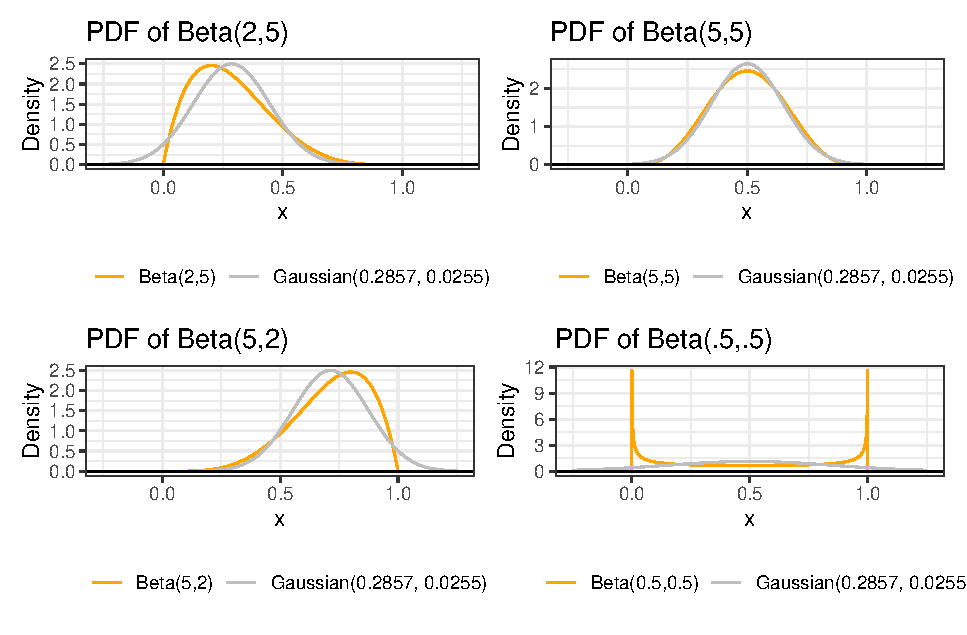
\includegraphics[scale=0.5]{densityf.pdf}
       \caption{}
     \label{densityf}
     \end{center}
   \end{figure}

\section{Properties}
There were four properties or moments, which we analyzed: mean, variance, skewness, and kurtosis. Moment are calculated using a given distribution and its parameters. In this lab, we calculated each value based on the beta distribution. Moments can either be un-centered, indicating that they take they don't account for the mean, or centered which means that they account for the mean. The moments are advantageous because they allow us to calculate the values for a sample. The equations are as follows. 


\[
\mu_X = \mathbb{E}(X)
\]

\[
\sigma_X^2 = \mathrm{var}(X) = \mathbb{E} \left[ (X - \mu_X)^2 \right]
\]

\[
\mathrm{skew}(X) = \frac{\mathbb{E} \left[ (X - \mu_X)^3 \right]}{\left( \mathbb{E} \left[ (X - \mu_X)^2 \right] \right)^{3/2}}
\]

\[
\mathrm{kurt}(X) = \frac{\mathbb{E} \left[ (X - \mu_X)^4 \right]}{\left( \mathbb{E} \left[ (X - \mu_X)^2 \right] \right)^2} - 3
\]

We then calculated the cumulative moment for each of the four moments for 500 observations, which we obtained randomly from the beta distribution-- we repeated this process 48 times. For instance, if we were calculating the cumulative mean, then we would calculate the mean at every observation from zero to 500. We found through our calculations that the cumulative mean of each tract converges to the population (the black y-intercept line) value by 500 observations. 
This ultimately shows that the beta distribution can be modeled given a hundred or more observations that align with it. 

\section{Estimators}
  Although we analyzed the beta distribution in lab 07, we never established a method to find its parameter values for a given data set to apply it. In lab 08, we utilized two estimator methods in order to determine the alpha and beta values for the beta distribution given our data set. The first estimator method is MOM or Measure of Moments. A moment can be calculated based on the population and based on the parameters (alpha and beta). The number of moments that we choose to analyze is equal to the number of unknown variables. The goal of the Measure of Moments is to finds parameter value where the chosen moments are equal in both calculations. The second estimator is the Measure of Likelihood (MLE). MLE is based on the principle of likelihood and uses the probability density function. The probability density function displays the frequency that values occur with respect to other values in the data set or distribution (semantics vary between discrete and continuous data). Given a certain set of parameters, MLE creates a probability density function and uses the function to check the density (amount that values occur relative to others) for each value in the data set. The likelihood is then calculated by multiplying each density together. The parameters that produce the greatest likelihood model the distribution most effectively. One caveat is that we often use the log likelihood because the standard likelihood function becomes extremely close to zero. 

WHICH ESTIMATOR TO USE
AND SIGNIFIANCE OF THE TABLE (COMPARISON WITH MLE AND MOM OR ALSO FOR ALPHA AND BETA VALUES?)
\subsection{Example}
  In lab 08, we used the the point estimators with the beta distribution to model data about death rates in 2022. We plugged in 8 as alpha and 950 as beta for our initial values and then tracked the values that our MLE and MOM functions produced, which allowed us to graph them (figure 4) and make direct comparisons. Just visually you can see that both the MLE and MOM peak at just before 8 for alpha and around 940 for beta; however the MLE estimator method has sharper peaks for both the alpha and beta values, which suggests that MLE is more accurate. This finding is supported by the actual values in table 1. The bias is less than MOM's for both alpha and beta, it is more precise, and MLE has less of an mse. Since the MLE is better with every indicator, it is safe to conclude that it is more effective for representing a population. 
  
\[
\text{bias} = \text{mean}(\text{distribution}) - \text{actual mean}
\]

\[
\text{variance} = (\text{standard deviation})^2
\]

\[
\text{precision} = \frac{1}{\text{variance}(\text{distribution})}
\]

\[
\text{mean squared error (MSE)} = \text{variance}(\text{distribution}) + \text{bias}^2
\]

  
  WHAT DOES THIS TELL US ABOUT WHICH TO USE?
  When we created our plot comparing the actual death rates in 2022 to the MLE and MOM estimations, we found that they were all distributed very similarly. The MLE and MOM distributions were practically identical and the population histogram followed a very similar shape to the lines. 



We used data about the death rates worldwide in 2022. We cleaned the data using the tidyverse \citep{tidyverse} 
and made it usable for a beta distribution (having every value between 0 and 1 inclusive). 
Since our overall goal was to compare the MLE and MOM, we calculated the values for each estimation  
method using R. We also created a graph using ggplot \citep{ggplot2} comparing the population distribution in a histogram to the MLE and 
MOM which were different colored lines.
After working with the data from the worldwide death rates, we created 1000 samples of data using set seed 
so that we could calculate that alpha and beta values for each point estimation method. Using the 1,000 
values for MLE alpha, MLE, beta, MOM alpha and MOM beta, we were able to create graphs that compared the MLE 
to the MOM.
death rates in from almost every part of the world in 2022. This 
Describe the data you are working with, if applicable. Describe the specific process you will follow to answer the question at hand. This does not mean you should write something like this.

%%%%%%%%%%%%%%%%%%%%%%%%%%%%%%%%%%%%%%%%%%%%%%%%%%%%%%%%%%%%%%%%%%%%%%%%%%%%%%%%
% Bibliography
%%%%%%%%%%%%%%%%%%%%%%%%%%%%%%%%%%%%%%%%%%%%%%%%%%%%%%%%%%%%%%%%%%%%%%%%%%%%%%%%
\vspace{2em}

\noindent\textbf{Bibliography:} Note that when you add citations to your bib.bib file \emph{and}
you cite them in your document, the bibliography section will automatically populate here.

\begin{tiny}
\bibliography{bib}
\end{tiny}
\end{multicols}

%%%%%%%%%%%%%%%%%%%%%%%%%%%%%%%%%%%%%%%%%%%%%%%%%%%%%%%%%%%%%%%%%%%%%%%%%%%%%%%%
% Appendix
%%%%%%%%%%%%%%%%%%%%%%%%%%%%%%%%%%%%%%%%%%%%%%%%%%%%%%%%%%%%%%%%%%%%%%%%%%%%%%%%
\newpage
\onecolumn
\section{Appendix}
\begin{table}[ht]
\centering
\begin{tabular}{rlrrr}
  \hline
 & Element & Bias & Precision & MSE \\ 
  \hline
1 & Alpha (MLE) & 0.07 & 2.13 & 0.48 \\ 
  2 & Beta (MLE) & 9.11 & 0.00 & 7132.70 \\ 
  3 & Alpha (MOM) & 0.08 & 1.83 & 0.55 \\ 
  4 & Beta (MLE) & 10.29 & 0.00 & 8288.46 \\ 
   \hline
\end{tabular}
\end{table}
If you have anything extra, you can add it here in the appendix. This can include images or tables that don't work well in the two-page setup, code snippets you might want to share, etc.

\end{document}
